\chapter{Interpretation}\label{Kap4}

Das folgende Kapitel dient der Bewertung und Einordnung der ermittelten Messwerte. Dazu werden zun"achst die Messwerte f"ur alle RPi-Nodes powered vs. nur aktive RPi-Nodes powered verglichen. Anschlie\ss end werden sie den Messwerten des RPi-Einzelrechners gegen"ubergestellt, sowohl den selbst ermittelten als auch den bisher publizierten. Abschlie\ss end werden eine Einordnung in die Top500-Liste vorgenommen und Grenzen des Versuchsaufbaus diskutiert. 

\section{HPLinpack/Bramble}\label{Interpretation-Linpack}

Tabellen \ref{fig:hpl5} und \ref{fig:hpl6} stellen die Messergebnisse f"ur beide Ausf"uhrungen von HPLinpack gegen"uber: 

\begin{figure}[htb]
  \centering
  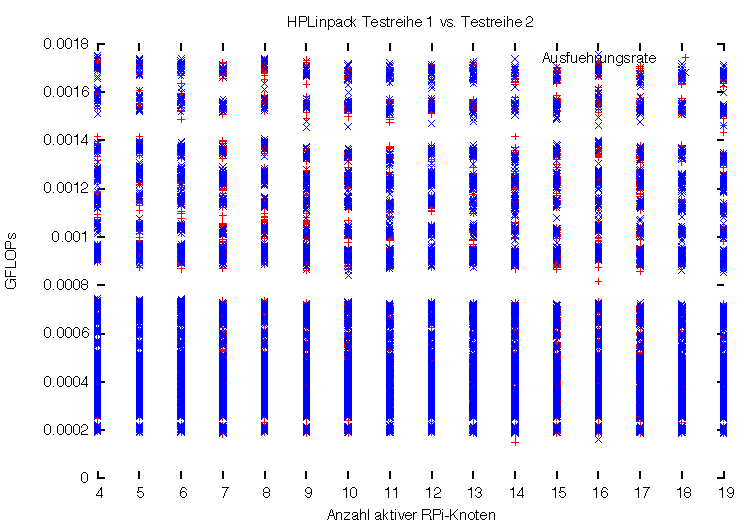
\includegraphics[scale=.8]{hpl5.pdf}\\ 
  \caption{Ausf"uhrungsrate in GFLOPS f"ur HPLinpack mit allen RPi-Nodes powered vs. nur aktive RPi-Nodes powered.}\label{fig:hpl5}
\end{figure}
\newpage
\begin{figure}[htb]
  \centering
  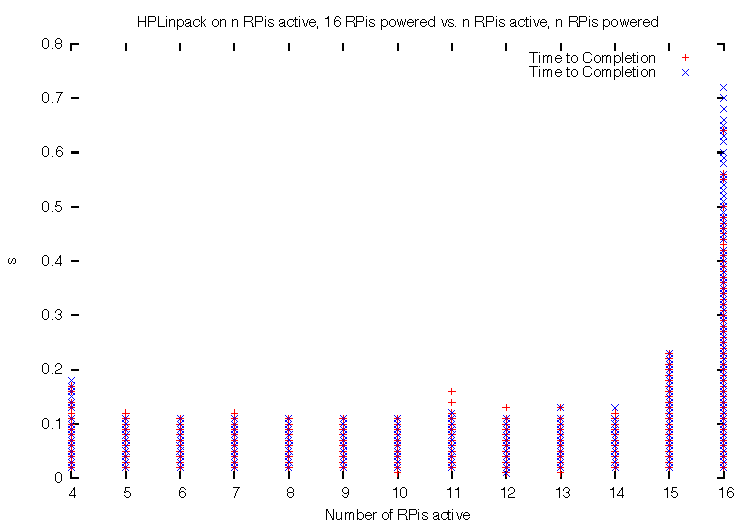
\includegraphics[scale=.8]{hpl6.pdf}\\ 
  \caption{Ausf"uhrungszeit in s f"ur HPLinpack alle RPi-Nodes powered vs. nur aktive RPi-Nodes powered.}\label{fig:hpl6}
\end{figure}

\noindent
Die Diagramme lassen vermuten, dass keine signifiganten Unterschiede zwischen der Ausf"uhrung von HPLinpack auf n RPi-Nodes aktiv/16 RPi-Nodes powered (rot) und n RPi-Nodes aktiv/n RPi-Nodes powered (blau) bestehen. Die folgende Tabelle stellt die minimalen, maximalen und durchschnittlichen Werte f"ur Ausf"uhrungsrate und Ausf"uhrungsdauer beider L"aufe gegen"uber: 

\begin{figure}[h!]
  \centering
  \begin{tabular}{|l|c|c|}
    \hline 
     & \textbf{16 RPis powered} & \textbf{n RPis powered}\\ 
    \hline 
    \textbf{Ausf"uhrungsrate/Min:} & 3.65E-05 GFLOPS & 3.01E-05 GFLOPS \\
    \hline 
    \textbf{Ausf"uhrungsrate/Max:} & 1.71E-03 GFLOPS & 1.73E-03 GFLOPS \\
    \hline 
    \textbf{Ausf"uhrungsrate/Avg:} & 5.10E-04 GFLOPS & 5.15E-04 GFLOPS \\
    \hline 
    \textbf{Ausf"uhrungsdauer/Min:} & 0.01 s & 0.01 s \\
    \hline 
    \textbf{Ausf"uhrungsdauer/Max:} & 0.64 s & 0.72 s \\
	\hline 
    \textbf{Ausf"uhrungsdauer/Avg:} & 0.07 s & 0.07 s\\
    \hline
  \end{tabular}
  \caption{Gegen"uberstellung HPLinpack alle RPis powered vs. nur aktive RPis powered.}\label{fig:hpl-vgl}
\end{figure}
\noindent
Leichte Unterschiede zeigen sich somit in der mimimalen, maximalen und durchschnittlichen Ausf"uhrungsrate sowie der maximalen Ausf"uhrungszeit. Dabei "uberschreitet die Abweichung nur bei der minimalen Ausf"uhrungsrate sowie der maximalen Ausf"uhrungszeit die Gr"o\ss enordnung einer Nachkommastelle. 

Hieran ist von Bedeutung, dass das Herunterfahren nicht aktiver RPi-Nodes lediglich bei der maximalen und durchschnittlichen Ausf"uhrungsrate einen positiven Effekt erzielt. Die "ubrigen Abweichungen zeigen sogar einen negativen Effekt: Die mimimale Ausf"uhrungsrate sinkt um 6.40E-06 = 0.0000064 GFLOPS, die durchschnittliche Ausf"uhrungsrate um 5.00E-06 = 0.0000050 GFLOPS und die maximale Ausf"uhrungsdauer steigt um 0.08 s. 

\section{STREAM/Bramble}\label{Interpretation-Stream}

Noch deutlicher zeigt sich dieser Effekt bei STREAM: 

\begin{figure}[h!]
  \centering
  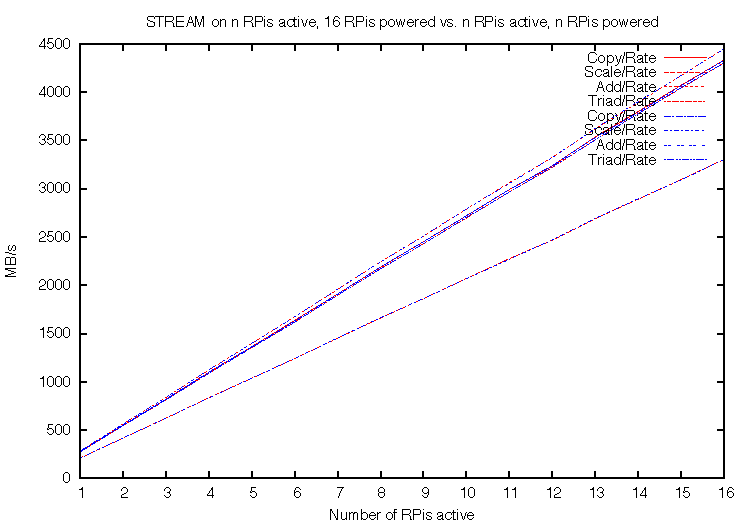
\includegraphics[scale=.8]{stream5.pdf}\\ 
  \caption{Ausf"uhrungsrate in MB/s f"ur STREAM alle RPi-Nodes powered vs. nur aktive RPi-Nodes powered.}\label{fig:stream5}
\end{figure}
\begin{figure}[htb]
  \centering
  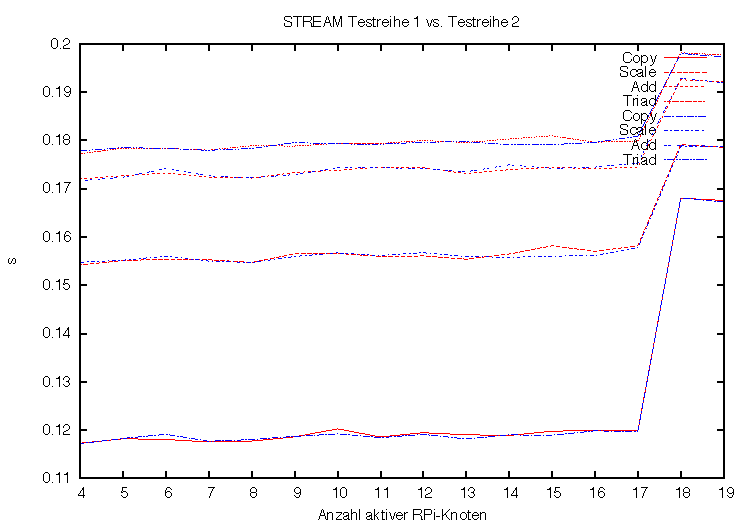
\includegraphics[scale=.8]{stream6.pdf}\\ 
  \caption{Ausf"uhrungszeit in s f"ur STREAM alle RPi-Nodes powered vs. nur aktive RPi-Nodes powered.}\label{fig:stream6}
\end{figure}

Auch hier zeigen die nahezu deckungsgleichen Ergebnisdaten mit 16 RPis powered (rote) vs. n RPi-Nodes powered (blau), keinen  nennenswerten Effekt des Herunterfahrens nicht aktiver RPi-Nodes auf Ausf"uhrungsrate und Ausf"uhrungsdauer. Die folgenden Tabellen \ref{fig:stream-vgl1} und \ref{fig:stream-vgl2} mit der Gegen"uberstellung der maximalen, minimalen und durchschnittlichen Ausf"uhrungsrate und Ausf"uhrungsdauer der STREAM-Module best"atigen dies: 

\begin{figure}[htb]
  \centering
  \begin{tabular}{|l|c|c|}
    \hline 
    & \textbf{16 RPis powered} & \textbf{n RPis powered}\\ 
    \hline 
    \textbf{Copy/Rate Min:} & 278.0 MB/s & 278.2 MB/s \\
    \hline 
	\textbf{Copy/Rate Max:} & 4330.0 MB/s & 4326.2 MB/s \\
    \hline
    \textbf{Copy/Rate Avg:} & 2310.5 MB/s & 2309.4 MB/s \\
 	\hline 
   	\textbf{Scale/Rate Min:} & 210.4 MB/s & 210.2 MB/s \\
   	\hline
   	\textbf{Scale/Rate Max:} & 3301.2 MB/s & 3301.5 MB/s \\
 	\hline 
   	\textbf{Scale/Rate Avg:} & 1757.2 MB & 1757.3 MB/s \\
 	\hline 
 	\textbf{Add/Rate Min:} & 283.2 MB/s & 282.9 MB/s \\
 	\hline 
   	\textbf{Add/Rate Max:} & 4447.1 MB/s & 4443.5 MB/s \\
  	\hline 
   	\textbf{Add/Rate Avg:} & 2367.4 MB/s & 2368.1 MB/s \\
 	\hline 
   	\textbf{Triad/Rate Min:} & 274.0 MB/s & 274.1 MB/s\\
 	\hline 	
   	\textbf{Triad/Rate Max:} & 4300.0 MB/s & 4298.9 MB/s \\
 	\hline 
   	\textbf{Triad/Rate Avg:} & 2292.9 MB/s & 2293.4 MB/s \\
   	\hline
 	\end{tabular}
  \caption{Gegen"uberstellung STREAM (Ausf"uhrungsrate) alle RPis powered vs. nur aktive RPis powered.}\label{fig:stream-vgl1}
\end{figure}

\begin{figure}[htb]
  \centering
  \begin{tabular}{|l|c|c|}
    \hline 
	& \textbf{16 RPis powered} & \textbf{n RPis powered}\\ 
    \hline 
    \textbf{Copy/Time Min:} & 0.115415 s & 0.115293 s \\
    \hline 
    \textbf{Copy/Time Max:} &  0.119951 s & 0.119217 s \\
    \hline
    \textbf{Copy/Time Avg:} & 0.118210 s & 0.118054 s \\
 	\hline 
   	\textbf{Scale/Time Min:} & 0.152540 s & 0.152485 s \\
 	\hline 
   	\textbf{Scale/Time Max:} & 0.157763 s & 0.155317 s \\
 	\hline 
 	\textbf{Scale/Time Avg:} & 0.155374 s & 0.155317 s \\
 	\hline 
   	\textbf{Add/Time Min:} & 0.169977 s & 0.1710393 s \\
  	\hline 
   	\textbf{Add/Time Max:} & 0.174637 s & 0.175129 s \\
 	\hline 
   	\textbf{Add/Time Avg:} & 0.172898 s & 0.172851 s \\
 	\hline 	
   	\textbf{Scale/Time Min:} & 0.176024 s & 0.175788 s \\
 	\hline 
   	\textbf{Scale/Time Max:} & 0.179734 s & 0.179793 s \\
 	\hline 
 	\textbf{Scale/Time Avg:} & 0.178582 s & 0.178587 s \\
 	\hline
 	\end{tabular}
  \caption{Gegen"uberstellung STREAM (Ausf"uhrungszeit) alle RPis powered vs. nur aktive RPis powered.}\label{fig:stream-vgl2}
\end{figure}

Unterschiede in der Gr"o\ss enordnung von mehr als einer Nachkommastelle zeigen sich in der maximalen und durchschnittlichen Ausf"uhrungsrate von COPY, der minimalen und maximalen Ausf"uhrungsrate von ADD, der maximalen und durchschnittlichen Ausf"uhrungsrate von TRIAD. Bei der Ausf"uhrungsdauer unterscheiden sich beide Runs in fast allen Werten geringf"ugig, jedoch nur in einer Funktion (minimale Ausf"uhrungsdauer f"ur ADD) in mehr als vier Nachkommastellen. Wenn man in Betracht zieht, dass HPLinpack f"ur die Ausf"uhrungsdauer Werte lediglich auf zwei Nachkommastellen genau ausgibt, sind diese Abweichungen bis auf letztgenannte vernachl"assigbar. 

Die Abweichungen sind auch hier nur teilweise erwartungsgem"a\ss : Lediglich die durchschnittliche Ausf"uhrungsrate f"ur TRIAD sinkt beim Herunterfahren nicht aktiver RPi-Nodes um 0.5 MB/s. Maximale und durchschnittliche Ausf"uhrungsrate f"ur COPY, minimale und maximale Ausf"uhrungsrate f"ur ADD und maximale Ausf"uhrungsrate von TRIAD sinken gegen"uber der Ausf"uhrung mit 16 RPi-Nodes powered.  Die Steigerung der minimalen Ausf"uhrungsdauer von ADD um 0.001062 s gegen"uber 16 RPi-Nodes zeigt ebenfalls einen negativen Effekt des Herunterfahrens.

Schlussfolgernd l"asst sich feststellen, dass das Herunterfahren nicht aktiver RPi-Nodes wie bei HPLinpack keinen nennenswerten Einfluss auf Ausf"uhrungsrate und Ausf"uhrungsdauer der STREAM-Module hat. 

\section{Vergleich Bramble/RPi-Einzelrechner}\label{Vergleich}

Eine Gegen"uberstellung der Messwerte von Bramble und RPi-Einzelrechner ist nur mit Einschr"ankungen m"oglich. Wie bereits dargestellt bestehen gro\ss e Unterschiede zwischen den Betriebssystemen und den verwendeten Implementierungen der Benchmarks, die zudem teilweise unterschiedliche Ergebnisparameter haben. Tabellen \ref{fig:overall1}, \ref{fig:overall2} und \ref{fig:overall3} stellen die Ergebnisse von Linpack, Whetstone und STREAM auf Bramble, RPi-Einzelrechner den Ergebnissen der Benchmark-Autoren\footnote{Quellen: \url{http://www.roylongbottom.org.uk/Raspberry\%20Pi\%20Benchmarks.htm} und \url{http://www.cs.virginia.edu/stream/stream_mail/2012/0002.html}.} gegen"uber.

%\footnote{Soweit ermittelbar, vgl. Kap. . Mit "`Linpack"' ist HPLinpack f"ur den Bramble und Linpack 100 f"ur die RPi-Einzelrechner gemeint. Ausf"uhrungsrate und Ausf"uhrungsdauer auf dem Bramble sind als Mittelwerte angegeben. Die Ergebniswerte wurden jeweils auf die geringste Genauigkeit der vorhandenen Messdaten gerundet.} 
\newpage
\begin{figure}[h!]
  \centering
  \begin{tabular}{|l|c|c|c|c|}
    \hline 
	& \textbf{Bramble/16} & \textbf{Bramble/n} & \textbf{RPi} & \textbf{RPi/Autor} \\ 
    \hline 
    \textbf{Ausf"uhrungsrate:} & 0.00051 & 0.00052 GFLOPS & 0.04131 GFLOPS & 0.04184 GFLOPS \\
	\hline	
 	\end{tabular}
  \caption{Linpack auf Bramble und RPi-Einzelrechnern.}\label{fig:overall1}
\end{figure}

\begin{figure}[h!]
  \centering
  \begin{tabular}{|l|c|c|c|c|}
    \hline 
	& \textbf{Bramble/16} & \textbf{Bramble/n} & \textbf{RPi} & \textbf{RPi/Autor} \\ 
    \hline 
    \textbf{Ausf"uhrungsrate:} & -- & -- & 255.154 MWIPS & 270.460 MWIPS \\
    \hline
    \textbf{Ausf"uhrungsdauer:} & -- & -- & 10.190 s & 9.983 s \\
    \hline
    \end{tabular}
  \caption{Whetstone auf RPi-Einzelrechnern.}\label{fig:overall2}
\end{figure}

\begin{figure}[h!]
  \centering
  \begin{tabular}{|l|c|c|c|c|}
    \hline 
	& \textbf{Bramble/16} & \textbf{Bramble/n} & \textbf{RPi} & \textbf{RPi/Autor} \\ 
    \hline 
    \textbf{Copy/Rate:} & 2310.5 MB/s & 2309.4 MB/s & 274.4 MB/s & 209.5 MB/s \\    
    \hline
    \textbf{Copy/Avg time:} & 0.11821 s & 0.1181 s & 0.5868 s & 0.1549 s \\
    \hline
    \textbf{Scale/Rate:} & 1757.2 MB/s & 1757.3 MB/s & 209.3 MB/s & 190.1 MB/s \\
    \hline
    \textbf{Scale/Avg time:} & 0.1554 s & 0.1553 s & 0.7664 s & 0.1703 s \\
    \hline
    \textbf{Add/Rate:} & 2367.4 MB/s & 2368.1 & 287.2 MB/s & 259.1 MB/s \\
    \hline
    \textbf{Add/Avg time:} & 0.1729 s & 0.1729 s & 0.8381 s & 0.1943 s \\
    \hline
    \textbf{Triad/Rate:} & 2292.9 MB/s & 2293.4 MB/s & 271.1 MB/s & 248.8 MB/s \\
    \hline
    \textbf{Triad/Avg time:} & 0.1786 s & 0.1786 s & 0.8868 s & 0.2002 s \\
    \hline  
    \end{tabular} 
  \caption{STREAM auf Bramble und RPi-Einzelrechnern.}\label{fig:overall3}
\end{figure}

\section{Einordnung in Top500}\label{top500}

Die Klassifizierung der Supercomputer in der Top500-Liste basiert auf den Ergebnissen von HPLinpack (Ausf"uhrungsrate in GFLOPS). Eine fiktive Einordnung des Bramble in die aktuelle Bestenliste vom November 2013\footnote{Vgl. \url{http://www.top500.org/list/2013/11}.} zeigt Schaubild \ref{fig:top500}.
\begin{figure}[h!]
  \centering
  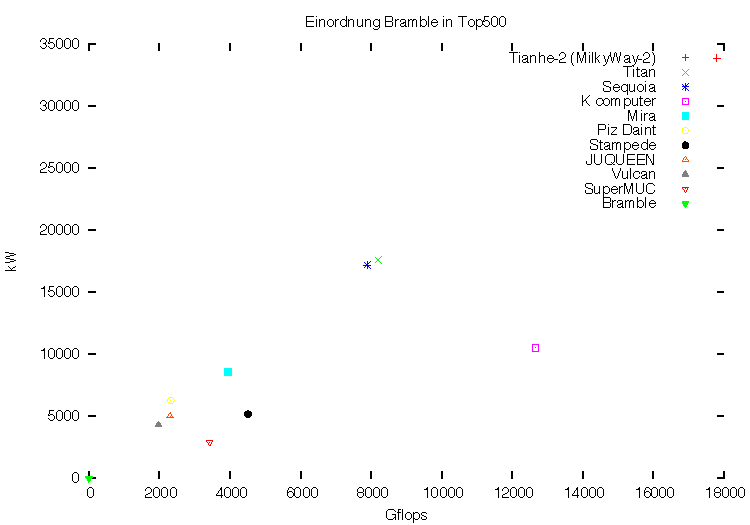
\includegraphics[scale=.8]{top500.pdf}\\ 
  \caption{Einordnung des Bramble in Top500 Nov. 2013.}\label{fig:top500}
\end{figure}

\section{Grenzen des Versuchsaufbaus}\label{Grenzen}
Der dargestellte Versuchsaufbau st"o\ss t in drei Bereichen an seine Grenzen: 
\begin{enumerate}
	\item \textbf{Vergleichbarkeit der Benchmark-Implementierungen}\\ 
Die ausgew"ahlten Benchmarks liefern teilweise h"ochst unterschiedliche Parameter als R"uckgabewerte, je nachdem ob eine MPI-Implementierung oder eine Single-CPU-Imple\-mentierung verwendet wird. Das gilt besonders f"Ur Linpack: Einziger R"uckgabewert f"ur Linpack 100 ist die Ausf"uhrungsrate in MFLOPS, w"ahrend HPLinpack f"ur jeden der 864 Tests Ausf"uhrungsrate in GFLOPS und Ausf"uhrungsdauer in s zur"uckgibt. Messwerte unterschiedlicher Implementierungen, die notwendigerweise auf einem Cluster und einem Einzelrechner verwendet werden, sind daher nur bedingt aussagekr"aftig. STREAM hingegen unterscheidet nicht zwischen den Ausgabewerten seiner unterschiedlichen Implementierungen, was die Vergleichbarkeit deutlich verbessert. 
	\item \textbf{Vergleichbarkeit des Benchmark-Designs}\\
Auch zwischen den Designs der Benchmarks bestehen gro\ss e Unterschiede. Whetstone in der gew"ahlten, an den RPi-Einzelrechner angepassten Implementierung liefert nach wie vor lediglich Ergebnisse in MWIPS. STREAM liefert standardm"a\ss ig Durchschnittswerte f"ur die Ausf"uhrungszeit jedes Moduls. HPLinpack testet deutlich mehr Module als die vorgenannten Benchmarks, liefert jedoch nur Einzelergebnisse f"ur Ausf"uhrungsrate und -dauer, keine Mittelwerte. Vergleichbarkeit zwischen den Ergebnissen unterschiedlicher Benchmarks ist daher noch weniger gegeben als zwischen den verschiedenen Implementierungen eines Benchmarks, selbst wenn sie dieselbe Komponente testen. 

Das gilt insbesondere f"ur HPLinpack zum Tragen. Die in Kap. \ref{Interpretation-Linpack} dargestellten Abweichungen sind deutlich geringer als die unterschiedlichen Ergebnisse der einzelnen Module einer einzigen Ausf"uhrung auf n RPi-Nodes. Auch wenn das dem Design des Benchmarks vorgesehen ist, ist die Interpretation an Hand selbst ermittelter Mittelwerte sicherlich weniger aussagekr"aftig als eine Interpretation von Mittelwerten als Teil des Designs. 
	\item \textbf{Zuverl"assigkeit von Hardware, IP- und SSH-Kommunikation des Bramble}\\
Schlie\ss lich erweist sich das Setup des RPi-Clusters als limitierender Faktor. Auch nach weitestgehendem Ausschluss aller in Kap. \ref{Bramble-Versuchsaufbau} genannten St"orfaktoren blieb der Versuchsaufbau fehleranf"allig. Die Durchf"uhrung erforderte i.d.R. die Anwesenheit einer Aufsichtsperson, um bei St"orungen die LEDs zu kontrollieren, Kabel zu "uberpr"ufen etc.. Der aktuelle Status Bramble kann kaum als stabil bezeichnet werden und es ist nicht auszuschlie\ss en, dass Fehlerf"alle stellenweise Einfluss auf die Messergebnisse nehmen. 

Erschwerend kommt hinzu, dass sich die RPi-Nodes des Bramble beim Herunterfahren anders verhalten als die eines RPi-Einzelrechners. Dieser schickt beim Aufruf von \texttt{shutdown} eine Broadcast-Message, dass das System jetzt heruntergefahren wird. Der Rechner kann sicher vom Stromnetz getrennt werden, wenn nur noch die rote Status-LED f"ur die Stromversorgung leuchtet.  

Beim Bramble hingegen sind alle Status-LEDs weiterhin aktiv, auch wenn der RPi-Node nicht mehr auf ein \texttt{ping} reagiert, d.h. keine IP-Verbindung vom Server oder einem anderen RPi-Node aus aufgebaut werden kann. Der Broadcast einer Shutdown-Nachricht wurde nur nur gelegentlich festgestellt. Somit erscheint es schwierig, den Zeitpunkt festzustellen, an dem ein RPi-Node tats"achlich vom Netz gegangen ist. Der aktuelle Versuchsaufbau d"urfte hierdurch jedoch nicht beeintr"achtigt werden: Auch wenn die Status-LEDs weiterhin aktiv sind, ist der Rechner nicht mehr durch \texttt{ping} zu erreichen und somit nicht mehr im Netzwerk aktiv. 
\end{enumerate}
\endinput 
% Seit einigen Jahren zeigt sich auch in der HPC-Welt ein zunehmendes Problembewusstsein betreffend den Energieverbrauch und -effizienz der verwendeten und untersuchten Systeme. Daraus resultiert das Green500-Ranking, das seit dem Jahr 2006 die Kandidaten der TOP500-Liste unter dem Aspekt der Energieeffizienz untersucht. Die Bestenliste liefert die Supercomputer mit dem besten Verh"altnis zwischen Leistung und Stromverbrauch (FLOPS pro Watt)\footnote{Vgl. \url{http://www.green500.org/}.}.
% Quelle: \url{http://www.green500.org/docs/pubs/RunRules_Ver1.0.pdf}